%%%%% The Solution %%%%%

\chapter{Proposed Solution: A New Teaching Environment for Programming} \label{ch_pa}

In order to let students have a \emph{Sichtenwechsel} with relation to programming, \ie have them experience several different abstraction layers involved between a program's source code and its execution, a new teaching environment dubbed ``Processing Abstractions'' is proposed:

Within \ac{GT}, we've implemented support for the Processing programming language and molded views for every implementation step along the way. This allows for creating interactive notebook pages containing source code and a variety of these views, showing \eg the \ac{AST} and resulting bytecode for the \ac{GT} \ac{VM} side-by-side.

In this chapter, we document the architecture of this environment and the reasons for the approaches chosen. If you want to inspect the environment yourself, see appendix \ref{app_setup} for how to install all referenced code\footnote{Remove the line \ct{GtExplorationHomeSection studentMode: true.} in order to also see our implementation notes.}



\section{Overview of ``Processing Abstractions''}

``Processing Abstractions'' consists of a transpiler for translating Processing source code into executable objects, a runtime environment, a large collections of views into various aspects of the program, and teaching materials using them.\footnote{The teaching materials currently provided are in the language used for teaching at the location of writing: German.} Tools and views as well as materials are all implemented within \acf{GT}, the former in Smalltalk code and the latter as ``Lepiter'' notebook pages.

\begin{cfigure}[fig_screenshot_vm_execution]{Excerpt from an interactive notebook page on program execution in a \ac{VM}.}
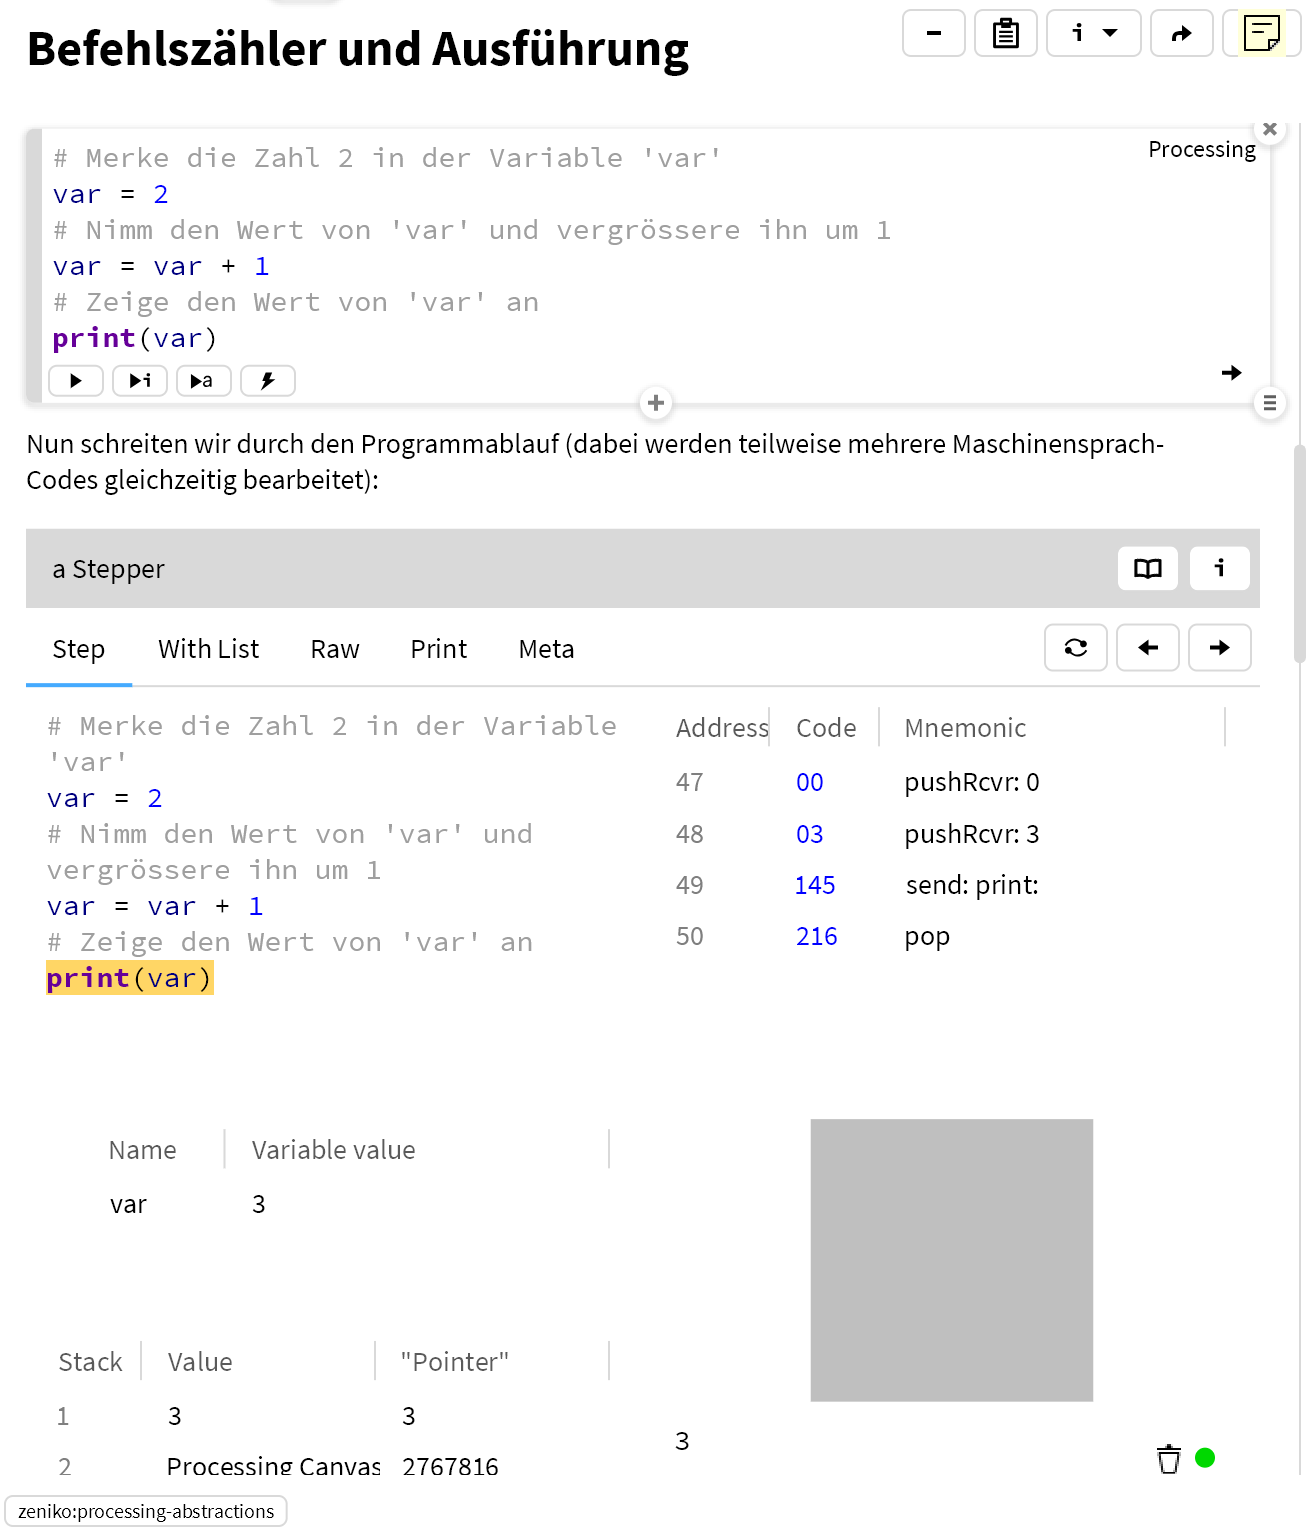
\includegraphics[width=.7\textwidth]{screenshot_vm_execution}
\end{cfigure}

Figure \ref{fig_screenshot_vm_execution} shows an excerpt from materials for students: The program visible at the top resides in a Processing-specific `snippet' with commands for running and inspecting the program independently of the page it resides on at the bottom; below a combined view for one execution step is shown with (clockwise) the step in question highlighted in source code; the corresponding bytecode visible; the program's output up to and including the current step; the contents of the execution stack of the Smalltalk \ac{VM}; and a list of all variable states.

Many such views are updated live whenever the source code is modified, without any other action required by students.\footnote{The one exception is the combined run-step view which for longer running programs would be too resource intensive to regenerate on the fly. Refreshing it manually is still possible.} The five views shown in figure \ref{fig_screenshot_vm_execution} can also be used on their own or in other arrangements (\eg only source and a full bytecode view where interacting with one automatically highlights the corresponding items in the other).

As will be shown below, dozens of premade views are available. Embedding any of them in a notebook page is done by adding an `Element' snippet with the one line of Smalltalk code shown in figure \ref{fig_embedding_view}. As an example, this code connects the first Processing snippet on the current page with a live \ct{gtTreePlusSourceFor:} view.

\begin{cfigure}[fig_embedding_view]{Smalltalk code for embedding a view in a notebook page}
\begin{code}
(ProcessingSource fromPage: thisSnippet page at: 1) renderLiveView: #gtTreePlusSourceFor:
\end{code}
\end{cfigure}

From these views, interactive teaching materials related to programming, compilers and code execution in a (virtual) machine can be composed, allowing students to combine their preexisting knowledge from programming with concepts of different abstraction layers.



\section{Exploring Abstraction Layers}

Any of the views into a program require its source written in Processing with Python syntax\footnote{Restricted to the implemented API as documented in appendix \ref{app_api}.} available either as a single file or as snippet in a \ac{GT} notebook. We recommend the latter, as views are then generally live and effects of changing the source code can be more easily explored by students.



\subsection{Source Snippet}

The ``Processing/Python'' snippet used in \ac{GT}'s notebook pages is the only place where Processing source code can be modified. It also provides several ways to run the program:

\begin{itemize}
\item {\small\faPlay} (or its shortcut \ct{Ctrl+R} for ``Run'') runs the program and either display its `Output' view or an inline error message.
\item {\small\faPlay}\texttt{i} (or its shortcut \ct{Ctrl+G} for ``debuG'') runs the program, recording all individual steps at the level of Python (sub)expressions -- allowing to step through the program's runtime views and inspecting among others the values of variables and the current state of the output.
\item {\small\faPlay}\texttt{a} (or its shortcut \ct{Ctrl+D} for ``Details'') shows the `Abstractions' view, \ie the program's main decomposition states: source code, \ac{AST}, bytecode, and output.
\item \lightning\ (or its shortcut \ct{Ctrl+Shift+D}) opens \ac{GT}'s Smalltalk debugger at the \ct{gtRun} entry point of the transpiled code for live debugging for either advanced students or for looking under the hood of the \ac{API} calls.
\end{itemize}

With just one source snippet, students can write and inspect programs with the opened views updating live as the program changes. This should give about the same experience as the Processing IDE with the main distinction that it's a live environment.

In contrast to the snippet, views are static in the sense that the source code can't be modified there.


\subsection{Output View}
% Source -> Output

The only views students should already know are the traditional `Source' and `Output' views which show the source code and the result of running the program respectively. Programs containing an animation loop will show the animation and allow user interaction in any output view.\footnote{Interactions are currently limited to mouse movements and clicks.}

The `Source' view is meant to be linked to any other view, allowing for interacting between them by selecting source expressions and having the corresponding item(s) in the other view(s) also selected.

The `Output' view can be used at any state to quickly verify visually that a program behaves as expected, be it during an introduction to programming or when exploring part of a program's execution or decomposition.\footnote{All of these views are directly available for a Processing program when running it using {\small\faPlay}\texttt{a} or \ct{Ctrl+D} and then selecting the \texttt{i} selector at the top (see figure \ref{fig_gt_screenshot} on page \pageref{fig_gt_screenshot}).}


\subsection{Compilation Views}
% Source -> Tokens -> AST -> Transpilation -> IR -> Bytecode

One way to show students what happens to a program before it can be executed on a (virtual) machine is to take them through the involved steps:

\begin{itemize}
\item The `Tokens` view (see figure \ref{fig_views_parser}) shows each of the tokens the lexer has encountered, including additionally required information such as a line number and line indentation\footnote{Indentation is relevant, as Python and as a consequence Processing with Python syntax is a language with significant whitespace, using common indentation for denotating code blocks.}. This view can be used for students to see what a compiler is looking at in their program with whitespace and comments in particular missing.\footnote{As a limitation, tokens are currently extracted in reverse from the parser which prevents inspecting tokens of syntactically invalid programs.}
\item The `\ac{AST}' view (see figure \ref{fig_views_parser}) shows the resulting parsing tree in a form that differentiates semantically relevant (sub)expressions from purely structural tokens. Combined with the `Tokens' view, this view can be used for hypothesizing and exploring how and what tokens are grouped together. In order to allow better interaction between `Tokens' and `\ac{AST}' views, the latter is a tree-list. A proper `\ac{AST} Tree' view is however also provided where the tree structure is more obviously visible, in particular also for larger programs.
\item The `Transpilation' view shows the result of translating the \ac{AST} to Smalltalk. Since the \ac{AST} needs to be barely modified for this translation step, Smalltalk code should be relatively easy to understand, at least when the original Processing source is displayed in parallel.

The `Transpilation' view also allows students to see what Processing does implicitly behind the scenes: setting and updating implicit variables, such as \ct{width}, \ct{mousePressed}, \etc, calling \ct{setup} once and \ct{draw} repeatedly, and running top-level code before entering the animation loop (see figure \ref{fig_animation_loop}).

In order to discuss programming language syntax, two additional views `Prefix' and `Postfix' show transpilations into a Lisp-like language using S-expressions and a Postscript-like language with reverse polish notation respectively. These may also serve as a basis for students' own parser projects, translating these pseudo-languages back into Processing or Smalltalk.
\item The `\acs{IR}' view shows the \ac{IR} generated by the Smalltalk Opal compiler from the transpiled Smalltalk code. With variable names still showing and optimizations still missing, this allows students to make more sense of the eventual bytecode, in particular when both views are displayed side-by-side.
\item The `Bytecode' view finally shows the bytecode which will be run by the Smalltalk \ac{VM}\footnote{Unless it's later translated to native code by the \ac{JIT}.} with instruction addresses\footnote{These are actually byte indices in the method's binary layout as used by the Smalltalk \ac{VM}.} and mnemonic added so that jumps can be understood and the code can be more easily connected to either \ac{IR} or any other form of Assembly language.
\end{itemize}

All of these views can be linked together, so that selecting an item in one view will highlight the corresponding item(s) in the linked views. The default `Abstractions' view, available directly from every Processing snippet, \eg combines the source with `\ac{AST}', `Bytecode' and `Output' (visible on the right hand side in figure \ref{fig_gt_screenshot} on page \pageref{fig_gt_screenshot}, with a source expression and its corresponding items highlighted).

\begin{cfigure}[fig_views_parser]{Screenshot of a page of student content showing modifyable Processing source with live views for tokenization (left) and abstract syntax tree (right).}
\centering
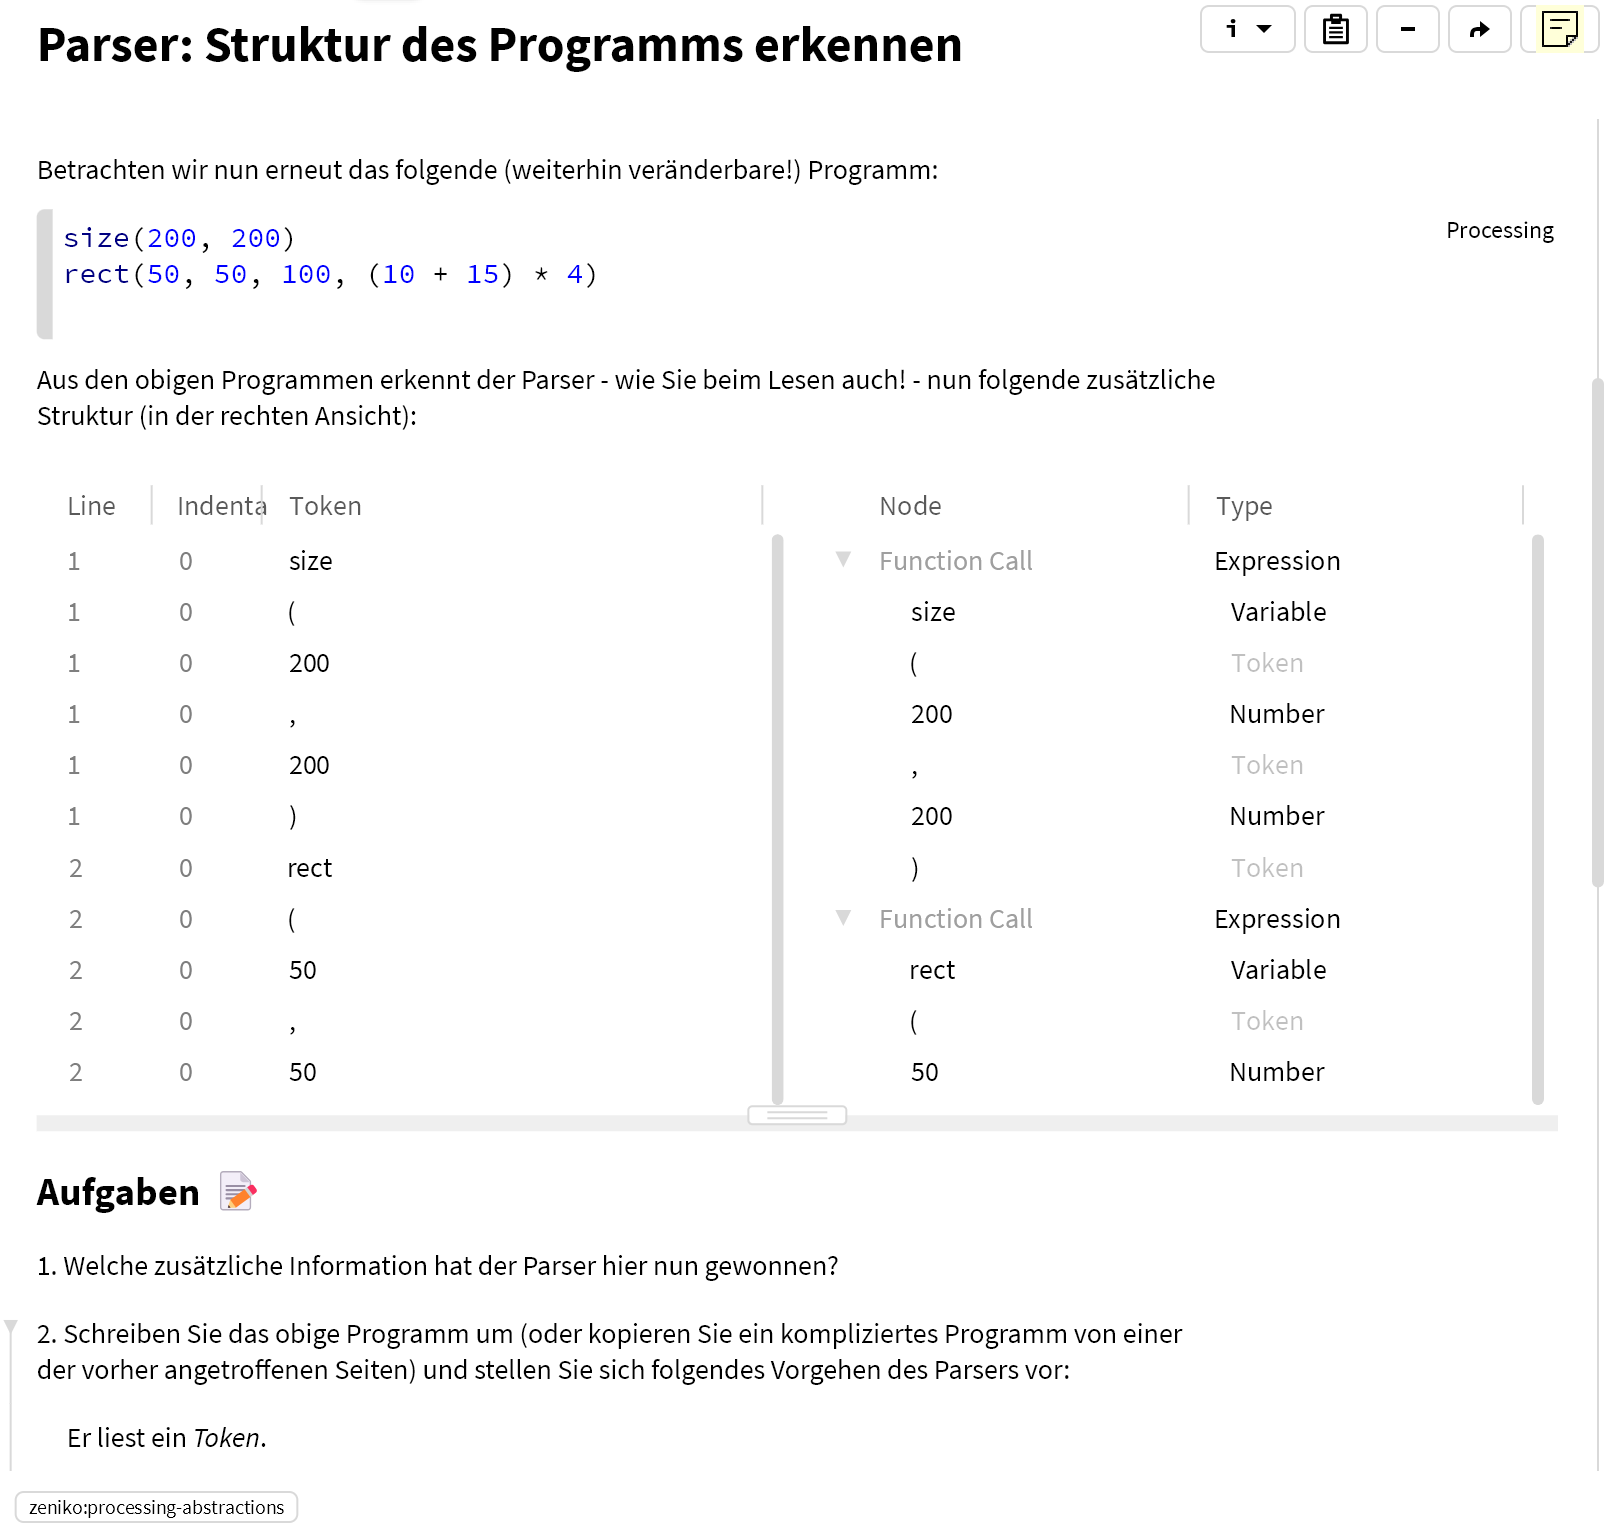
\includegraphics[width=.8\textwidth]{screenshot_parser}
\end{cfigure}

\begin{cfigure}[fig_animation_loop]{Implicit animation loop (Transpilation view) and part of the required \ac{API} (only visible when debugging transpiled code)}
\begin{code}
SubclassOfProcessingCodeBase >> gtRun
	self setup.
	[ gtCanvas frameRate > 0 ] whileTrue: [
		mouseX := gtCanvas mouseX. mouseY := gtCanvas mouseY.
		mousePressed := gtCanvas mousePressed.
		self draw.
		gtCanvas endFrame.
	].
\end{code}

\begin{code}
ProcessingCanvas >> endFrame [
	presenter updateOutput.
	(1 / frameRate) seconds wait.	"The frame rate is adjustable through `frameRate()`"
	frameCount := frameCount + 1.
	transform := #yourself	"Transforms are reset at the end of a draw-cycle"
]
\end{code}
\end{cfigure}


\subsection{Run Step Views}
% Run Step -> Source -> Bytecode -> Execution Stack -> Variables


Finally, there's three views tied to a program's runtime which may be helpful even for a pure introduction to programming: \ct{gtOutptFor:} shows the output of a program which may continuously change, if the program describes an animation, and which may be interacted with\footnote{For now only using the mouse which changes the implicit variables \ct{mouseX}, \ct{mouseY} and \ct{mousePressed} and calls the callbacks \ct{mousePressed}, \ct{mouseReleased}, \ct{mouseClicked} and \ct{mouseMoved} if any of them has been defined by the user.}; \ct{gtOutputShapesFor:} allows inspecting the individual shapes in the order they've been rendered (this view is disabled for animations); and \ct{gtStepsFor:} shows an overview of all views of \ct{ProcessingRunStep} for every Processing (sub)expression that has been evaluated -- including the expression in the source, the transpilation and its bytecode form, current variable values, values on the Smalltalk \ac{VM}'s stack and the current output state. This gives us a debugging view in which a student can step forward and backward through the execution of the program but also shows an excerpt of the different layers involved in program execution.


\subsection{Source Data}
% Source -> Characters -> Bytes

At the level of source code, there's three different views showing the source with syntax highlighting (\ct{gtContentsFor:}), showing the individual source characters with their unicode value (\ct{gtSourceCharsFor:}), and showing the bytes as they would be written to disk, assuming the default UTF-8 encoding also used by the original Processing \ac{IDE}, with bytes also displayed in hexadecimal and binary notations (\ct{gtSourceBytesFor:}). With these views and suitable sample code, students might be able to deduce some regularities with relation to ASCII character ranges and UTF-8 encoding.


\subsection{Other Views}
% Source -> Slices
% Source -> Shapes



\section{Implementation Details}


\subsection{Views}

All views in \ac{GT} are by convention provided by methods with names of the form \ct{gt...For:} and are categorized as ``views'' in the class browser.\footnote{Actual requirement is only the \ct{<gtView>} pragma annotation and the method signature (\ct{GtPhlowView} $\rightarrow$ \ct{GtPhlowView}).}

With any view visible in \ac{GT}, \ct{Alt}+clicking on a view's name shows its source method(s), revealing the view's method name and implementation. The method name will be required for embedding a view in a notebook page as described in figure \ref{fig_embedding_view} above.

For comparing the same views of different programs, the \ct{ViewComparison} helper class is provided which can be used in `Element' snippets as follows:

\begin{code}
ViewComparison newFor: {
	(ProcessingSource fromPage: thisSnippet page at: 1) program -> #gtSourceCharsFor:.
	(ProcessingSource fromPage: thisSnippet page at: 2) program -> #gtSourceCharsFor:.
}
\end{code}


Any of these views can be integrated on its own into an interactive notebook page for producing student content, they are however also all available to students through the Processing/Python snippet's various execution modes: Either running the program for pure output ({\small\faPlay} or \ct{Ctrl+R}) gives access to the most common views by inspecting the object behind the output ({\small\faPlay}\texttt{i} in the upper right corner); or running the program for details ({\small\faPlay}\texttt{a} or \ct{Ctrl+D}) yields all the views through \texttt{i} at the top center. For manageability, both of these options can be ignored at the start, as the default views should provide sufficient informations and the remaining ones can be continually introduced during class.


\section{Classes}

%%%%% The Solution (UML Diagram) %%%%%

\newgeometry{bottom=1cm}

\begin{landscape}

\begin{cfigure}[fig_uml_processing]{Diagram of most classes involved in running Processing code within \ac{GT}}

\begin{tikzpicture}

\begin{package}{Processing}

\begin{class}[text width=6cm]{ProcessingSource}{0, 0}
\operation{fromFile:}
\operation{fromPage:at:}
\operation{fromSnippet:}
\end{class}

\begin{class}[text width=6cm]{ProcessingProgram}{0, 2.5}
\operation{ast}
\operation{compilation}
\operation{run}
\end{class}

\begin{class}[text width=6cm]{ProcessingParser}{-8, 0}
\operation{parse:}
\end{class}

\begin{class}[text width=6cm]{ProcessingTranspiler}{-8, 2.5}
\operation{transpile:}
\end{class}

\begin{class}[text width=6cm]{ProcessingTranspilationSlice}{-8, 7.5}
\operation{link:method:from:to:}
\end{class}

\begin{interface}[text width=6cm]{ProcessingCodeBase}{0, 5}
\operation{gtRun}
\end{interface}

\begin{class}[text width=6cm]{ProcessingRunner}{8, 5}
\operation{run:}
\operation{runSteps:}
\end{class}

\begin{class}[text width=6cm]{ProcessingCanvas}{0, 7.5}
\operation{asElement}
\operation{presenter}
\end{class}

\begin{class}[text width=6cm]{ProcessingCanvasPresenter}{8, 7.5}
\implement{ProcessingCanvas}
\end{class}

\begin{class}[text width=6cm]{ProcessingCanvasElement}{8, 9}
\end{class}

\begin{class}[text width=6cm]{ProcessingAstCleaner}{-8, 5}
\operation{clean:}
\end{class}

\begin{interface}[text width=6cm]{ProcessingCanvasShape}{0, 9}
\end{interface}

\begin{class}[text width=6cm]{ProcessingRunStep}{8, 2.5}
\end{class}

\draw[umlcd style dashed line, ->] (ProcessingSource) -- node[black]{$<<$accesses$>>$} (ProcessingProgram);
\draw[umlcd style dashed line, <->] (ProcessingProgram) -- node[black, sloped]{$<<$source $\rightarrow$ \ac{AST}$>>$} (ProcessingParser);
\draw[umlcd style dashed line, ->] (ProcessingProgram) -- node[black]{$<<$uses$>>$} (ProcessingTranspiler);
\draw[umlcd style dashed line, ->] (ProcessingTranspiler) -- node[black, sloped]{$<<$creates$>>$} (ProcessingCodeBase);
\draw[umlcd style dashed line, <->] (ProcessingTranspiler) -- node[black]{$<<$uses$>>$} (ProcessingAstCleaner);
\draw[umlcd style dashed line, ->] (ProcessingTranspiler.west) -- +(-1, 0) |- node[black, pos=0.25, sloped]{$<<$creates$>>$} (ProcessingTranspilationSlice);
\draw[umlcd style dashed line, ->] (ProcessingProgram) -- node[black]{$<<$accesses$>>$} (ProcessingCodeBase);
\draw[umlcd style dashed line, ->] (ProcessingProgram) -- node[black, sloped]{$<<$uses$>>$} (ProcessingRunner);
\draw[umlcd style dashed line, ->] (ProcessingRunner) -- node[black]{$<<$runs$>>$} (ProcessingCodeBase);
\draw[umlcd style dashed line, ->] (ProcessingRunner) -- node[black]{$<<$creates$>>$} (ProcessingRunStep);
\draw[umlcd style dashed line, ->] (ProcessingCodeBase) -- node[black]{$<<$owns$>>$} (ProcessingCanvas);
\draw[umlcd style dashed line, ->] (ProcessingRunner) -- node[black, sloped]{$<<$creates$>>$} (ProcessingCanvas);
\draw[umlcd style dashed line, ->] (ProcessingCanvas) -- node[black]{$<<$controls$>>$} (ProcessingCanvasPresenter);
\draw[umlcd style dashed line, ->] (ProcessingCanvasPresenter) -- node[black]{$<<$interacts$>>$} (ProcessingCanvasElement);
\draw[umlcd style dashed line, ->] (ProcessingCanvas) -- node[black]{$<<$creates$>>$} (ProcessingCanvasShape);
\draw[umlcd style dashed line, ->] (ProcessingCanvasShape) -- node[black]{$<<$renders$>>$} (ProcessingCanvasElement);

\end{package}

\end{tikzpicture}

\end{cfigure}

\end{landscape}

\restoregeometry


\ac{GT} was chosen for its moldable environment: As shown in \ref{sc_gt}, different views are quick to implement and can be combined freely with interactions and updates between them.

Since \ac{GT} is based on Smalltalk, an initial effort is required to learn language and environment before these benefits can be used. This is helped by Smalltalk's regular syntax and \ac{GT}'s reflective capabilities.\footnote{For Smalltalk and \ac{GT}'s ancestor Pharo, there are sufficient resources available online, for \ac{GT} itself, there's the ``Glamorous Toolkit Book'' \cite{Gir23} and a Discord server.}

Implementing a new language in \ac{GT} can happen along the moldable patterns documented in \ref{sc_moldable}: Starting with concrete samples, classes and views for handling them are molded in steps until the desired behavior is reached; then code is refactored into permanent methods on the one hand and a concrete example serving as test case on the other. Whenever the need for a different view into the program or one of its intermediary forms (such as \ac{AST}, bytecode or output) arises, the view is constructed in the same way by first iteratively shaping the data into the desired form and then either passing this to one of \ac{GT}'s standard views (text, list, tree, table, forward) or composing the view's layout in the same way iteratively.

The product consists of the following main classes which can be found in \ac{GT} through the spotter (\faSearch):

\ct{ProcessingCanvas} provides the implementation of most of the Processing \ac{API} for rendering the various shapes in the form of \ct{BlElement}s (wrapped through \ct{ProcessingCanvasShape}). It does this through \ct{ProcessingCanvasPresenter} into a \ct{ProcessingCanvasElement} of which there can be multiple, allowing to use a canvas for multiple views. The canvas also provides access to the individual shapes and all of its state. Rendering onto the canvas happens through the transpiled and compiled Processing program for which a new canvas is created for every separate run.

Processing programs can be written either inside \ac{GT}'s notebook in form of a ``Processing/Python'' snippet, in form of a Smalltalk string or in separate files. All forms are loaded through the \ct{ProcessingSource} class. Since we mostly want Processing source and its various views to be seen in a notebook page, the most common way to process a Processing program will be inside the page through\footnote{The \ct{at: 1} part of the message may also be omitted, if there's only one snippet on a notebook page. Omit the \ct{renderLive} message, if you want access to any of the intermediary states or different views.}
\begin{code}
(ProcessingSource fromPage: thisSnippet page at: 1) renderLive
\end{code}




The snippet is implemented in \ct{LeProcessingSnippet} which builds upon \ac{GT}'s \ct{LePythonSnippet} for syntax highlighting but accesses Processing through \ct{ProcessingSource} instead of Python through \ct{PythonBridge}.

For embedding output or any other view inside a notebook page, an ``Element'' is added with either the code from above or with \ct{renderLive} replaced with \ct{renderLiveView:} with the symbol of the desired view appended (\ct{#gtTreeFor:}, \ct{#gtTranspilationFor:}, \ct{#gtBytecodeFor:}, \etc; see the ``views'' category of \ct{ProcessingSource} and \ct{ProcessingProgram} for all available views).

For all the views, a \ct{ProcessingProgram} is created through \ct{ProcessingSource>>>program} which transforms it into its various forms:

\begin{itemize}
\item \ct{ProcessingParser} is used for parsing the source into an \ac{AST}. Since Processing shares Python's syntax, the parser is a very thin wrapper around \ac{GT}'s \ct{PythonParser}. The \ac{AST} is then slightly modified through \ct{ProcessingAstCleaner} to better map Python to Smalltalk: Since statements after a \ct{return} are allowed in Python but not supported in Smalltalk, they're silently dropped (a warning about unreachable code could be added); and parenthesized expressions are parsed into \ct{PyTupleExpressionNode} which complicate later optimizations with relation to operator chains, in particular logical operators \ct{and} and \ct{or}.
\item \ct{ProcessingTranspiler} then walks through the cleaned \ac{AST} and transpiles Python expressions to the corresponding Smalltalk, recording a \ct{ProcessingTranspilationSlice} for every (sub)expression, thus later allowing to map bytecode its mapping into Smalltalk code back to the corresponding Processing source. If \ct{setup} and/or \ct{draw} functions are defined in Processing code, the implicit animation loop is added to the end of top-level code. Processing \ac{API} calls -- if not overwritten by user code -- are translated through messages of the form \ct{ProcessingTranspiler>>>emit_...:} which the transpiler detects through reflection.
\item The transpiled code is compiled to methods of an anonymous subclass of \ct{ProcessingCodeBase}. This base class provides views at the lower abstraction levels from transpiled code to bytecode and also the entry point to the user supplied program \ct{gtRun} which contains top-level code. Global variables are turned into instance variables, thus being available to all Processing functions in the form of Smalltalk methods.\footnote{In order to prevent overriding of \ct{gtRun} and the different view messages, Processing names starting with \ct{gt} are renamed to starting with \ct{gt_} during transpilation.}
\end{itemize}

While compiled Processing programs can be run directly, \ct{ProcessingRunner} is used for ensuring the presence of an output canvas, for allowing program execution to be interrupted and for extracting \ct{ProcessingRunStep} instances for every Processing (sub)expression.

From these, \ct{ProcessingProgram} provides all views corresponding to Processing code and combined views. In order not to overwhelm students with too many views, \ct{gtDefaultInspectorTool} has been implemented for hiding all but the main four views behind the same symbols as used by the snippet.

During compilation, most common exceptions are \ct{SmaCCParserError} during parsing, \ct{ProcessingCompileTimeException} during transpilation and \ct{ProcessingRunTimeException} during execution. At this point, exceptions occurring in the transpiled code are not translated yet. Since most programs are meant to be re-run live, a heuristic has been implemented for catching endless loops which may naturally occur while a program's source is modified where \eg a variable's value is modified but at the end of a \ct{while} loop. Instead of detecting the endless loop from code, runtime has been restricted to a maximum of two seconds for non-animated programs and thirty seconds for animated programs.



\section{Usage}

With this, high school teachers get a toolkit for teaching programming and systems at various levels:

At the start of a course, the environment can be used as an introduction to programming (see the suggested lessons in \ref{sc_lesson_intro}). When the limitations of the environment are reached, the move over to the official Processing \ac{IDE} should be seamless: code copied over and run (with the same icon and shortcut) yields the same output and can then be further modified with the full Processing \ac{API}, once students are ready.

When teaching computer architecture, the environment can be used for either exploring the various abstraction levels involved or even again as a full course embedded in notebook pages (see \ref{sc_lesson_ca}). In case of both usages, this better ties together programming and system architecture. And if programming has happened in Processing, students can investigate their own programs instead of mainly relying on those given by the teacher.

In an in-depth course for students specializing in computer science, this environment can further be used to teach the inner workings of a compiler from lexer to optimizer (see \ref{sc_lesson_compiler}).

Finally, this environment could also be used as a stepping stone for introducing Smalltalk as a different programming language and \ac{GT} as the moldable environment it is, leading students to molding the provided materials further by \eg extending the Processing \ac{API}, developing new views or starting to work on a language of their own (see \ref{sc_lesson_other}).

In all cases, \ac{GT} can also be used as a digital notebook by students, where they solve tasks directly in the page, add their own notes and keep their modified examples.

While this environment is mainly targetted at high school students, it could also be used in middle school. For middle schoolers, the exposed user interface would however have to be reduced as far as possible to keep it manageable. It could however work at least in a smaller group with interested and motivated students wanting to step beyond block based programming languages. For university students, there's currently not enough depth available.


\section{Other approaches considered}

A stable snapshot of the code discussed here is available at \url{https://github.com/zeniko/gt-exploration/tree/thesis}.

Within \ac{GT}, Processing is implemented through transpilation to Smalltalk. This allows reusing several of \ac{GT}'s libraries: \ct{PythonParser} for parsing Processing with Python syntax and \ct{OpalCompiler} for compiling Smalltalk with bytecode extractable through \ct{CompiledCode>>>symbolicBytecodes}.

Since Processing implemented on top of Python is a strongly but dynamically typed language, it maps well onto Smalltalk which is the same. Still, initially three other approaches were considered:

Processing could be run either in the original \ac{JVM} and then accessed through Python or directly run using one of several Python libraries \cite{Tab22}. In all cases, its objects would be accessed through \ct{PythonBridge}. Since at the time of writing, support for PythonBridge under Windows was difficult to achieve in a portable manner (\ie without requiring students to install multiple different packages which increases the risk of accidental breaking and thus potential support issues), this approach was rejected.

Alternatively, Processing could have been implemented through an interpreter in \ac{GT}\footnote{Remnants of which are available as \ct{ProcessingInterpreter}.}. This would have required to write a separate compiler for creating bytecode just for demonstration purposes. Instead, a compiler from Processing to Smalltalk bytecode could have been written.\footnote{A compiler for a tiny subset of Processing is included as \ct{ProcessingCompiler}.} While this would have allowed for closer control over optimizations, it would effectively have become a reimplementation of most of \ct{OpalCompiler}.



\section{Potential Drawbacks}

While Modrow and Strecker prefer a block based language, we feel that at least parts of their issue with a text based programming language can be remedied by having a live environment with custom error messages. For remedying their remaining issue about allowing individual bits of code to be called independently, that could be achieved in one of the ways \ac{GT} does this: either by offering separate playgrounds which do work similarly to a \ac{REPL}; by allowing multiple code snippets to access the same environment (as it also works in Jupyter notebooks); or by allowing only selected code to be executed. The last option would be easiest to implement.\footnote{It hasn't been implemented for three reasons: At least in the beginning, it might confuse students more than it helps, which goes against manageability (see \ref{ssc_manageability}); most visual commands can't be executed entirely independently in Processing, as output always depends on \ct{size} and maybe other stateful commands; and interaction with the animation loop would have to be figured out: whether it's has to be paused during the entire interaction, just between two user commands or even not at all.}

Chiodini \etal \cite{Chi23} also propose starting with visual programming but have different requirements: In order to keep an introductionary language manageable, they ask among others for a limited \ac{API} which should be expandable by students (see also \ref{ssc_manageability}). And the full Processing \ac{API} can indeed be quite overwhelming, so only a subset must be introduced at the start. Indeed also for this reason only a subset has been implemented in \ac{GT} (see appendix \ref{app_api}), although already including some seemingly unnecessary functions: \eg the \ct{circle} function is easily implemented in terms of the more generic \ct{ellipse} function (see figure \ref{fig_circle}) -- either in the implementation of the Processing \ac{API} or by students.

\begin{cfigure}[fig_circle]{Implementation of \ct{circle} as built-in \ac{API} and in user code}
\begin{minipage}{.5\textwidth}
\begin{code}
ProcessingCanvas >> circle: x y: y d: d
	self
		ellipse: d
		by: d
		at: x @ y
\end{code}
\end{minipage}
\begin{minipage}{.45\textwidth}
\begin{code}
def circle(x, y, d):
	ellipse(x, y, d, d)
\end{code}
\end{minipage}
\end{cfigure}

Another requirement by Chiodini \etal is for problems to be transparently decomposed and solutions recomposed. This is indeed an issue with Processing: Moving a composed shape to a different location requires adjusting the coordinates of all basic shapes involved, therefore variables and even functions have to be introduced sooner rather than latter to allow the examples shown \cite{Chi23} to work. Similar to how they introduce a library to achieve their desired \ac{API}, the same functionality could be implemented on top of Processing at a later stage if desired.\footnote{In the provided teaching materials, an example of how to implement a simpler Turtle based \ac{API} is provided (see ``Schildkr�ten und Rekursion'').}

The main reason for not introducing a new \ac{API} as proposed by Chiodini \etal is the same as the reason for not introducing an entirely new programming language optimized for teaching (as done \eg by Black and Bruce \cite{Bla18}): This prevents benefiting from the large community and preexisting documentation and example code.

\begin{todo}
\item Shorten ``Implemented Classes'', move the details into an appendix
\item Decide which screenshots belong into the appendix instead.
\item use 2DET taxonomy? \cite{Sor13}
\end{todo}
